\chapter{Background}

\section{Markov Decision Process}

Markov Decision Processes (MDPs) are a classical formalization of sequential decision making under uncertainty, where actions influence not just immediate responses, but also subsequent situations. Hence an MDP can be described as a controlled \textit{Markov chain}\footnote{A sequence of random variables $X_0, X_1, . . .$ with values in a countable set $S$ is a \textit{Markov chain} if at any time $n$, the future states (or values) $X\textsubscript{n+1}, X\textsubscript{n+2}, . . .$ depend on the history $X_0, . . . , X_n$ only through the present state $X_n$~\cite{konstantopoulos2009markov} .}, where the control is given at each step by the chosen action. In this chapter we will present the structure of an MDP and many techniques to solve its.

\paragraph{Markov Decision Process} Markov decision processes are defined as controlled stochastic processes satisfying the \textit{Markov property}\footnote{A stochastic process has the \textit{Markov property} if the probabilistic behaviour of the chain in the future depends only on its present value and discards its past behaviour.} and assigning reward values to state transitions~\cite{Put94}.  Formally, they are described by the 5-tuple ($S$, $A$, $T$, $p$, $r$) where:

\begin{itemize}
	\item $S$ is the state space in which the process’ evolution takes place;
	\item $A$ is the set of all possible actions which control the state dynamics;
	\item $T$ is the set of time steps where decisions need to be made;
	\item $p()$ denotes the state transition probability function;
	\item $r()$ provides the reward function defined on state transitions.	
\end{itemize}

\subparagraph{States} The set of environmental states $S$ is defined as the finite set $\{s_1, . . . , s_N\}$ where the size of the state space is $N$, i.e. $|S| = N$~\cite{wiering2012reinforcement}. Each state ${s \in S}$ is a vector of attributes (\textit{state variables}) that describes the current configuration of the system~\cite{Nevmyvaka}. More specifically, a state variable is the minimally dimensioned function of history that is necessary and sufficient to compute the "state of knowledge"~\cite{Powell}.

\subparagraph{Actions} The set of actions $A$ is defined as the finite set $\{a_1, . . . ,a_K\}$ where the size of the action space is $K$, i.e. $|A| = K$. Actions can be used to control the system state. The set of actions that can be applied in some particular state $s \in S$, is denoted $A(s)$, where $A(s) \subseteq A$. In more structured representations the fact that some actions are not applicable in some states, is modelled by a precondition function : $S$ × $A→{true,false}$, stating whether action $a \in A$ is applicable in state $s \in S$~\cite{wiering2012reinforcement}.

\subparagraph{Time Steps} The set of time steps $T$ is defined as the finite set $\{t_1, . . . ,t_M\}$ where the size of the action space is $M$, i.e. $|T| = M$.

\subparagraph{Transition Probability} The transition probabilities $p()$ characterize the state dynamics of the system, i.e. indicate which states are likely to appear after the current state. For a given action $a$, $p(s'|s,a)$ represents the probability for the system to transit to state $s'$ after undertaking action $a$ in state $s$. This $p()$ function is usually represented in matrix form where we write $P_a$ the $|S|$ x $|S|$ matrix containing elements $\forall s, s', P\textsubscript{a, s, s'} = p(s'|s,a)$. Since each line of these matrices sums to one, the $P_a$ are said to be stochastic matrices. The $p()$ probability distributions over the next state $s'$ follow the fundamental property which gives their name to Markov decision processes. If we write $h_t = (s_0, a_0, ..., s\textsubscript{t-1}, a\textsubscript{a-1}, s_t)$ the history of states and actions until time step $t$, then the probability of reaching state $s\textsubscript{t+1}$ consecutively to action $a_t$ is only a function of $a_t$ and $s_t$, and not of the entire history $h_t$~\cite{Sigaud:2010:MDP:1841781}. We can resume this concept through the following equation :

\begin{equation}
	\forall h_t, a_t, s\textsubscript{t+1} \quad P(s\textsubscript{t+1} | h_t, a_t) = P(s\textsubscript{t+1} | s_t, a_t) = p(s\textsubscript{t+1} | s_t, a_t)
\end{equation}

\subparagraph{Reward Function} The reward function specifies rewards for being in a state, or doing some action in a state. The state reward function is defined as $R : S \rightarrow \mathbb{R}$, and it specifies the reward obtained in states. The reward function is an important part of the MDP that specifies implicitly the \textit{goal} of learning. Thus, the reward function is used to give direction in which way the system, i.e. the MDP, should be controlled~\cite{wiering2012reinforcement}. It is critical that the rewards we set up truly indicate what we want accomplished. If we reward the achievement of subgoals , then the agent might find a way to achieve them without achieving the real goal. Reward signal is our way of communicating the agent \textit{what} we want to achieve, not \textit{how} it achieved~\cite{SuttonBarto}.

\begin{figure}[h!]
	\centering
	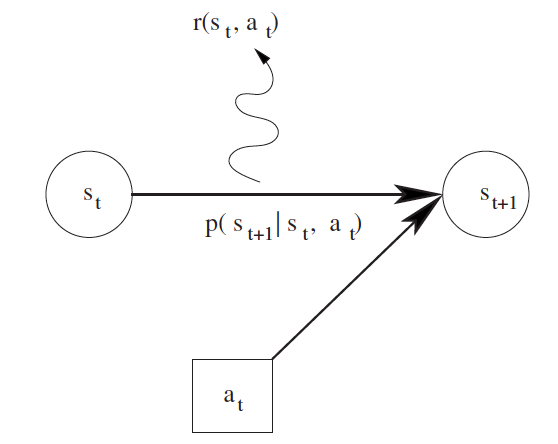
\includegraphics[width= 8cm, height = 7cm]{MDP.png}
	\caption{Markov decision process~\cite{Sigaud:2010:MDP:1841781}.}
	\label{fig:MDP}
\end{figure}

Markov decision processes allow us to model the state evolution dynamics of a
stochastic system when this system is controlled by an agent choosing and applying
the actions $a_t$ at every time step $t$. The procedure of choosing such actions is called
an action policy, or strategy, and is written as $\pi$~\cite{Sigaud:2010:MDP:1841781} .

\subparagraph{Policy} Formally, given an MDP $\bigl\langle S, A, p(), r() \bigr\rangle$, a policy is a computable function that outputs for each state $s \in S$ an action $a \in A(s)$~\cite{wiering2012reinforcement} A policy can decide deterministically upon the action to apply or can define a probability deistribution over the possible applicable actions. Then, a policy can be based on the whole history $h_t$ (history-dependent policy) or can only consider the current state $s_t$. Thus, we can obtain four main families policies, as shown in table \ref{table:T1}.

\begin{table}[h!]
\centering
\begin{tabular}{|c|c|c|}
	\hline Policy $\pi_t$
	&Deterministic &Stochastic  \\
	\hline 
	\hline Markov 
	&$s_t \rightarrow a_t$  &$a_t, s_t \rightarrow [0, 1]$ \\ 
	\hline History-dependent
	&$h_t \rightarrow a_t$  &$h_t, s_t \rightarrow [0,1]$  \\ 
	\hline 
\end{tabular}
\caption{Different policy families for MDPs~\cite{Sigaud:2010:MDP:1841781}}
\label{table:T1}
\end{table} 

For a deterministic policy, $\pi_t (s_t)$ or $\pi_t (h_t)$ defines the chosen action $a_t$. For a stochastic policy, $\pi_t (a, s_t)$ or $\pi_t (a, h_t)$ represents the probability of selecting $a \in A$ for $a_t$~\cite{Sigaud:2010:MDP:1841781}. The sets so defined are included in each other, from the most general case of stochastic, history-dependent policies, to the very specific case of deterministic, Markov policies, as shown in figure \ref{fig:Policies_schema}.

\begin{figure}[h!]
	\centering
	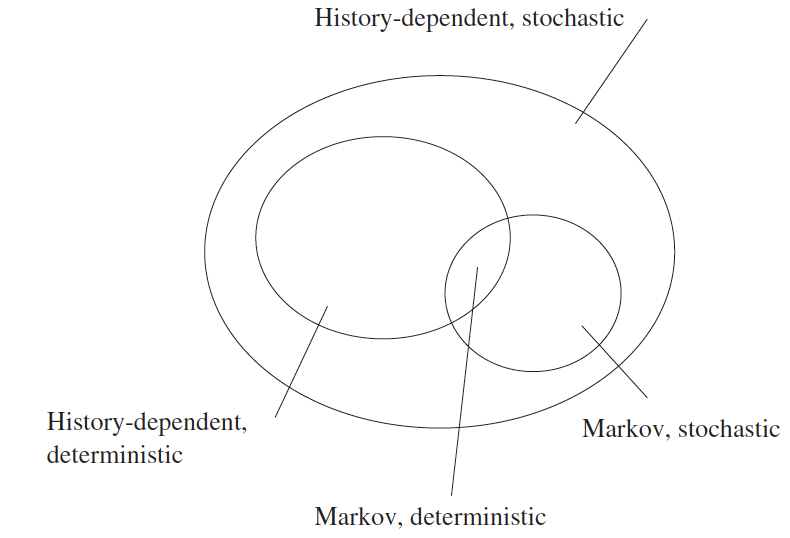
\includegraphics[width= 9cm, height = 7cm]{Policies_schema.png}
	\caption{Relationship between the different sets of policies~\cite{Sigaud:2010:MDP:1841781}.}
	\label{fig:Policies_schema}
\end{figure}

Application of a policy to an MDP is done in the following way. As shown in figure \ref{fig:Policy_application_schema} each time an agent performs an action $a\textsubscript{t}$ in a state $s\textsubscript{t}$, it receives a real-valued reward $t\textsubscript{t}$ that indicates the immediate value of this state-action transition. This produces a sequence of states $s\textsubscript{i}$, actions $a\textsubscript{i}$, and immediate rewards $r\textsubscript{i}$ as shown in the figure. The agent's task is to learn a control policy, $\{\pi : S \longrightarrow A\}$, that maximizes the expected sum of these rewards, with future rewards discounted exponentially by their delay~\cite{Mitchell}.

\begin{figure}[h!]
	\centering
	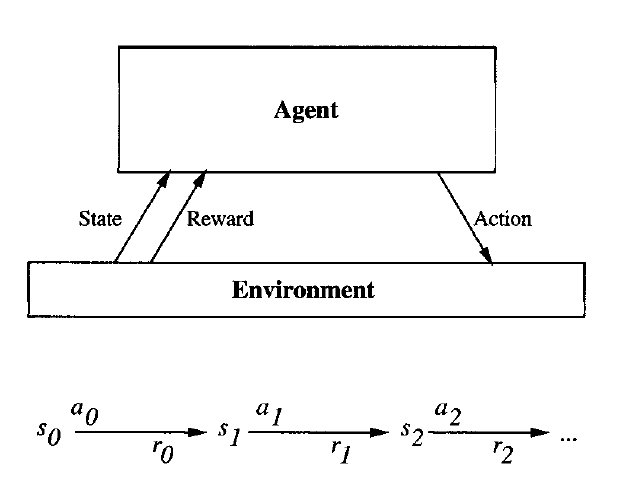
\includegraphics[width= 12cm, height = 10cm]{RLSchema.png}
	\caption{Policy application schema~\cite{SuttonBarto}.}
	\label{fig:Policy_application_schema}
\end{figure}

As already said the goal of learning in an MDP is to gather rewards. There are several ways of taking into account the future in how to behave now. There are basically three models of optimality in the MDP, which are sufficient to cover most of the approaches in the literature :

\begin{figure}[h!]
\begin{equation*}
E[\sum_{t = 0}^h r_t]
\qquad
E[\sum_{t = 0}^\infty \gamma^t r_t]
\qquad
\lim\limits_{h \rightarrow \infty} E[1/h \sum_{t = 0}^h r_t]
\end{equation*}
\caption{Optimality : \textbf{a)} finite horizon, \textbf{b)} discounted, infinite horizon, \textbf{c)} average reward}
\end{figure}

\subparagraph{Discount Factor}The \textit{finite horizon} model simply takes a finite horizon of length $h$ and states that the agent should optimize its expected reward over this horizon. In the \textit{infinite-horizon model}, the long-run reward is taken into account, but the rewards that are received in the future are discounted according to how far away in time they will be received.
A \textit{discount factor} $\gamma$, with $0 \leq \gamma \leq 1$ is used for this. Note that in this discounted case, rewards obtained later are discounted more than rewards obtained earlier. Additionally, the discount factor, ensures that, even with infinite horizon, the sum of the rewards obtained is finite. In episodic tasks, i.e. in tasks where the horizon is finite, the discount factor is not
needed or can equivalently be set to $1$. If $\gamma = 0$ the agent is said to be myopic, which means that it is only concerned about immediate rewards.
The last optimality model is \textit{average-reward} model, maximizing the long-run \textit{average-reward}. Sometimes this is called the \textit{gain optimal} policy and in the limit, it is equal to the infinite-horizon discounted model~\cite{wiering2012reinforcement}

\subparagraph{Bellman Equation} The concept of \textit{value function} is the link between optimality criteria and policies. Most learning algorithms for MDPs compute optimal policies by learning value functions. The value of a state $s$ under policy $\pi$, denoted $V^\pi (s)$ is the expected return when starting in $s$ and following $\pi$ thereafter. Using the infinite-horizon, discounted model :

\begin{equation}
	V^\pi (s) = E_\pi \{\sum_{k = 0}^{\infty} \gamma^k t\textsubscript{t+k} | s_t = s\}
\end{equation}

A similar state-action value function : $Q : S$ x $A \rightarrow \mathbb{R}$ can be defined as the expected return starting from state $s$. taking action $a$ and thereafter following policy $\pi$ :

\begin{equation} \label{eq:2.2}
	Q^\pi (s,a) = E_\pi\{\sum_{k = 0}^{\infty} \gamma^k r\textsubscript{t+k} | s_t = s, a_t = a\}
\end{equation}

For any policy $\pi$ and any state $s$ the expression \ref{eq:2.2} can recursively be defined in terms of a so-called \textit{Bellman Equation} :

\begin{equation}
\begin{split}
	V^\pi (s) = E_\pi\{r_t + \gamma\textsubscript{t+1} + \gamma^2 r\textsubscript{t+2} + ... | s_t = t\} \\
	= E_\pi \{r_t + \gamma V^\pi(s\textsubscript{t+1}) | s_t = s\} \\
	\sum_{s'}T(s, \pi(s), s') (R(s, a, s') + \gamma V^\pi (s'))
\end{split}	
\end{equation}

It denotes that the expected value of state is defined in terms of immediate reward and values of possible next state weighted by thei transition probabilities, and additionally a discount factor. Note that multiple policies can have the same value function, but for a given policy $\pi$, $V^\pi$ is unique. The goal for any MDP is to find a best policy, i.e. the policy that receives the most reward. This means maximizing the value function of equation \ref{eq:2.2} for all states $s \in S$. An optimal policy, denoted $\pi^*$, is such that $V\textsuperscript{$\pi$*} (s) \geq V^\pi (s)$ for all $s \in S$ and all policies $\pi$ :

\begin{equation} 
\label{eq:2.5}
V^*(s) = \max_{a \in A} \sum_{s'}T(s, \pi(s), s') (R(s, a, s') + \gamma V^\pi (s'))
\end{equation}

This expression is called the \textit{Bellman optimality equation}. It states that the value of a state under an optimal policy must be equal to the expected return for the best action in a state~\cite{wiering2012reinforcement}.

\section{Solving MDP}

Now that we have defined MDPs, policies, optimality criteria and value functions, it is time to consider the question of how to compute optimal policies. As already said, solving an MDP means computing an optimal policy $\pi^*$. Several dimensions exists along which algorithms have been developed for this purpose. The most important distinction is that between \textit{model-based} and \textit{model-free} algorithms ~\cite{wiering2012reinforcement}.
\begin{table}[h!]
	\resizebox{\textwidth}{!}{ 
		\begin{tabular}{|c|c|c|}
			\hline 
			&\textbf{Model-based algorithms}  &\textbf{Model-free algorithms}  \\ 
			\hline \textbf{General name} 
			&DP  &RL  \\ 
			\hline \textbf{Basic assumption} 
			&\thead{A model of the MDP is known \\ beforehand, and can be used to compute \\ value functions and policies using \\ the Bellman equation.}  &\thead{They rely on interaction with the environment. \\ Because a model\\ of the MDP is not known, \\ the agent has to explore the MDP to obtain \\ information.}  \\
			\hline 
		\end{tabular} 
	}
	\caption{Main differences between model-based and model-free algorithms.}
\end{table}

\subparagraph{Dynamic Programming} The term DP refers to a class of algorithms that is able to compute optimal policies in the presence of a perfect model of the environment~\cite{wiering2012reinforcement}. The method of dynamic programming systematically records solutions for all sub-problems of increasing lengths. According to Bellman optimality principle, all optimal sub-policies of an optimal policy are optimal sub-policies. Using this programming paradigm the optimal policy is defined through the step-by-step definition of optimal sub-policies.
The assumption that a model is available will be hard to ensure for many applications, however DP algorithms are very relevant because they define fundamental computational mechanism which are also used when no model is available.




\section{The nature of Reinforcement Learning}

\paragraph{} Reinforcement Learning (RL) is the problem faced by a learner that must behavior through trial-and-error interactions with a dynamic environment. It can be considered a problem of mapping situations to actions in order to maximize a numerical reward signal~\cite{RLDef1}.

\paragraph{} In RL the learner must select an action to take in each time step: every choice done by the agent changes the environment in an unknown fashion and receives a reward which value is based on the consequences. The objective of the learner is to choose a sequence of actions based on observations of the current environment that maximizes cumulative reward or minimizes cumulative cost over all time steps~\cite{LiMalik}.

\paragraph{} RL is different both from \textit{supervised learning} and from \textit{unsupervised learning}. It is not a sample of learning from a training set of labelled examples provided by a knowledgeable external supervisor (\textit{supervised learning}) and it is not a sample of searching and finding structure hidden in a collection of unlabelled data (\textit{unsupervised learning}). More specifically we can say that RL can be distinguished from other forms of learning based on the following characteristics :

\begin{itemize}
  \item Reinforcement Learning deals with temporal sequences. In contrast with non-supervised learning problems where the order in which the examples are presented is not relevant, the choice of an action at a given time step will have consequences on the examples that are received at a subsequent time steps~\cite{Sigaud:2010:MDP:1841781}.
  \item In contrast with supervised learning, the environment does not tell the agent what would be the best possible action. Instead, the agent may just receive a scalar reward representing the value of its action and it must \textit{explore} the possible alternative actions to determine whether its action was the best or not~\cite{Sigaud:2010:MDP:1841781}.
\end{itemize}

According to what just said, one of the challenges that arise in RL, and not in other kind of learning, is the trade-off between \textit{exploration} and \textit{exploitation}. To obtain an higher reward, an RL agent must prefer actions that it has tried in the past and found to be effective in producing reward. In order to discover such actions, it has to try actions that it has not selected before. The agent \textit{exploits} what it has already experienced in order to obtain reward, but it has also to \textit{explore} in order to eventually make better action selections in the future~\cite{SuttonBarto}. In other words \textit{exploitation} consists of doing again actions which have proven fruitful in the past, whereas \textit{exploration} consists of trying new actions, looking for a larger cumulated reward, but eventually leading to a worse performance. Dealing with the exploration/exploitation trade-off consists of determining how the agent should explore to get as fast as possible a policy that is optimal or close enough to the optimum~\cite{Sigaud:2010:MDP:1841781}.

\section{Elements of reinforcement learning}

\paragraph{} In RL the learner and decision maker is called the \textit{agent}. The thing it interacts with, comprising everything outside the agent, is called the \textit{environment}. It is described by some set of possible \textit{states} (\textit{S}). The agent can perform any of a set of possible \textit{actions} (\textit{A}). Each state ${s \in S}$ is a vector of attributes (\textit{state variables}) that describes the current configuration of the system~\cite{Nevmyvaka}. More specifically, a state variable is the minimally dimensioned function of history that is necessary and sufficient to compute the "state of knowledge"~\cite{Powell}.

Except for the \textit{agent} and for the \textit{environment} one can identify four other main sub-elements: 

\begin{itemize}
  \item the \textit{policy} : defines the learning agent's way of behaving at a given time (a mapping from states to actions).
  \item the \textit{reward signal} : defines the goal in a RL problem. On each time step, the environment sends to the RL agent a single number called the \textit{reward}. The agent's sole objective is to maximize the total reward it receives over the run. 
  \item the \textit{value function} : specifies the total amount of reward an agent can expect to accumulate over future, starting from a specific state.
  \item the \textit{model} : allows inferences to be made about how the environment will behave.
\end{itemize}

\begin{figure}[h!]
\centering
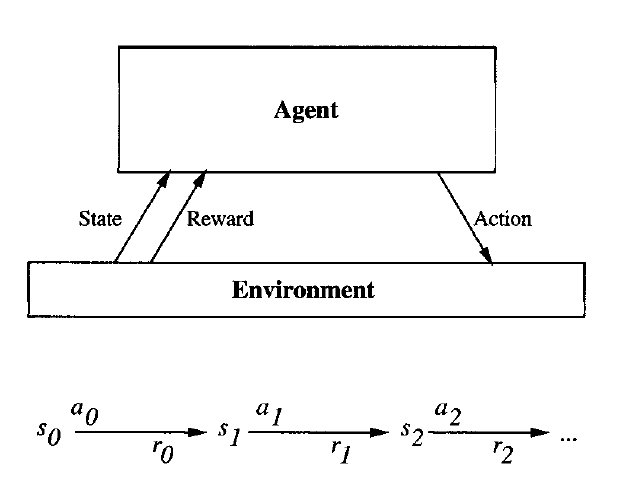
\includegraphics[width= 12cm, height = 10cm]{RLSchema.png}
  \caption{RL working schema.}
  \label{fig:RLWS}
\end{figure}

As shown in figure \ref{fig:RLWS} each time an agent performs an action $a\textsubscript{t}$ in a state $s\textsubscript{t}$, it receives a real-valued reward $t\textsubscript{t}$ that indicates the immediate value of this state-action transition. This produces a sequence of states $s\textsubscript{i}$, actions $a\textsubscript{i}$, and immediate rewards $r\textsubscript{i}$ as shown in the figure. The agent's task is to learn a control policy, $\{\pi : S \longrightarrow A\}$, that maximizes the expected sum of these rewards, with future rewards discounted exponentially by their delay~\cite{Mitchell}.

\paragraph{} According to how just said, the most important feature distinguishing RL from other types of learning is that it uses training information that \textit{evaluates} the actions taken rather than \textit{instructs} by giving correct actions. It is clearly an \textit{on-line learning} technique (data arrives sequentially and the model is continually updated as new data becomes available).

\section{Finite Markov Decision Processes}

\paragraph{} The environment in RL problems can be well described as \textit{Markov decision processes} (MDPs). MDPs are a classical formalization of sequential decision making under uncertainty, where actions influence not just immediate rewards, but also subsequent situations, or states, and through those future rewards. From a similar perspective we can define MDPs as a general mathematical formalism for representing shortest path problems in stochastic environments.

\paragraph{} A MDP process relies on the notation of state at time $t$, $S_t$, the action selected on time $t$, $A\textsubscript{t}$, the corresponding reward $R\textsubscript{t}$. The value of an arbitrary action $a$, denoted $q\textsubscript{*}(a)$ is the expected reward given that $a$ is selected : $q\textsubscript{*}(a) = \mathbb{E}[ R\textsubscript{t}|A\textsubscript{t} = a ]$. We denote the estimated value of an action $a$ at time step $t$ as $Q\textsubscript{t}(a)$.

\paragraph{} Solving an MDP consists
of controlling the agent in order to reach an optimal behaviour, i.e. to maximize its overall revenue. Because action effects are stochastic and, thus, can result in different possible states at the next stage of the decision process, the optimal control strategy cannot necessarily be represented as a single sequence of actions. Due to the uncertainty in actions’ results, applying a given policy can result in different sequences of states/actions~\cite{Sigaud:2010:MDP:1841781}.


\subsection{The Agent-Environment Interface}
\paragraph{} In MDPs the agent and environment interact at each of a sequence of discrete time steps, $t = 0, 1, 2, 3, 4, ...$. At each time step $t$, the agent receives some representation of the environment's $state$, $S\textsubscript{t} \in S$, and on that basis selects an $action$, $A\textsubscript{t} \in A(s)$. One time step later, in part as a consequence of its action, the agent receives a numerical $reward$, $R\textsubscript{t+1} \in R \subset \mathbb{R}$, and finds itself in a new state, $S\textsubscript{t+1}$. The MDP and agent together thereby give rise to a sequence of $trajectory$ that begins like this :
\begin{equation}
S\textsubscript{0}, A\textsubscript{0}, R\textsubscript{1}, S\textsubscript{1}, A\textsubscript{1}, R\textsubscript{2}, S\textsubscript{2}, A\textsubscript{2}, R\textsubscript{3}, S\textsubscript{3}, A\textsubscript{3}, ...
\end{equation}

\paragraph{} In a $finite$ MDP, the set of states, actions and rewards ($S, A, R$) all have a finite number of elements. In this case, the random variables $R\textsubscript{t}$ and $S\textsubscript{t}$ have well defined discrete probability distributions dependent only on the preceding state and actions. That is, for particular values of these random variables, $s' \in S$ and $r \in R$, there is a probability of those values occurring at time $t$, given particular values of the preceding state and action : 

\begin{equation}
p(s', r | s, a) = Pr\{S\textsubscript{t} = s', R\textsubscript{t} = r | S\textsubscript{t-1} = s, A\textsubscript{t-1} = a\}
\end{equation}

for all $s'$, $s \in S$, $r \in R$, and $a \in A(s)$. The function $p : S$ x $R$ x $S$ x $A \longrightarrow [0, 1]$ is an ordinary deterministic function of four arguments~\cite{SuttonBarto}. The '$\mid$' in the middle of it just reminds us that $p$ specifies a probability distribution for each choice of $s$ and $a$ :

\begin{equation}
  \sum_{s'\in S} \sum_{r\in R} p(s', r | s, a) = 1,  \forall s \in S, a \in A(s). 
\end{equation}

\begin{center}

  \begin{figure}[h!]
  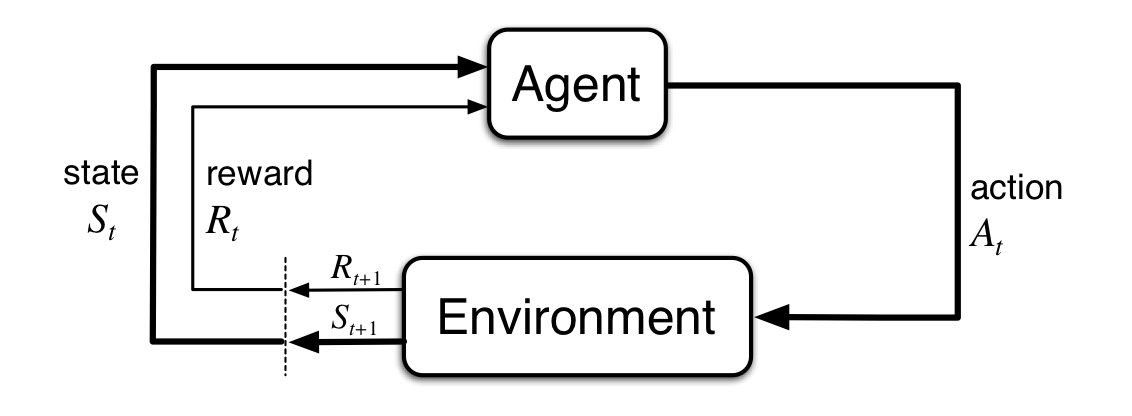
\includegraphics[width= 15cm, height = 6.5cm]{MDPSchema.png}
    \caption{The agent-environment interaction in a MDP.}
    \label{fig:MDPS}
  \end{figure}
  
\end{center}

This type of decision process is called a Markov process because it obeys the \textit{Markov property}. In systems that obey this property, the future of the system is independent of its past, given the current state. In other words, if we know the current state, knowing additional information about previous states and reinforcements does not improve our ability to predict future states or reinforcements~\cite{Maia2009}.


\subsection{Goals, Rewards, Returns and Episodes}
\paragraph{} As previous said, in RL, the goal of the agent is to maximize the expected value of the cumulative sum of a received scalar signal called \textit{reward}. It is critical that the rewards we set up truly indicate what we want accomplished. If we reward the achievement of subgoals , then the agent might find a way to achieve them without achieving the real goal. Reward signal is our way of communicating the agent \textit{what} we want to achieve, not \textit{how} it achieved. 

\paragraph{}Let's suppose that the sequence of rewards received after time step $t$ is denoted $R\textsubscript{t+1}$, $R\textsubscript{t+2}$, $R\textsubscript{t+3}$, $R\textsubscript{t+4}$, $...$. We expect the agent maximizes the \textit{expected return}, where the return, denoted $G_t$, is defined as some specific function of the reward sequence. In the simplest case the return is the sum of the rewards :

\begin{equation}
  G_t = R\textsubscript{t+1} + R\textsubscript{t+2} + R\textsubscript{t+3} + R\textsubscript{t+4} + ... + R_T, 
\end{equation}

where $T$ is a final time step. This approach make sense in  applications in which there is a natural notion of final time step, that is, when the agent-environment interaction breaks naturally into subsequences, which we call \textit{episodes} (\textit{E})~\cite{SuttonBarto}. To be more specific, in this case, the breaking into subsequences is also visible in episodes and we call them \textit{epochs} (\textit{e}). 

\begin{center}
  \begin{figure}[h!]
  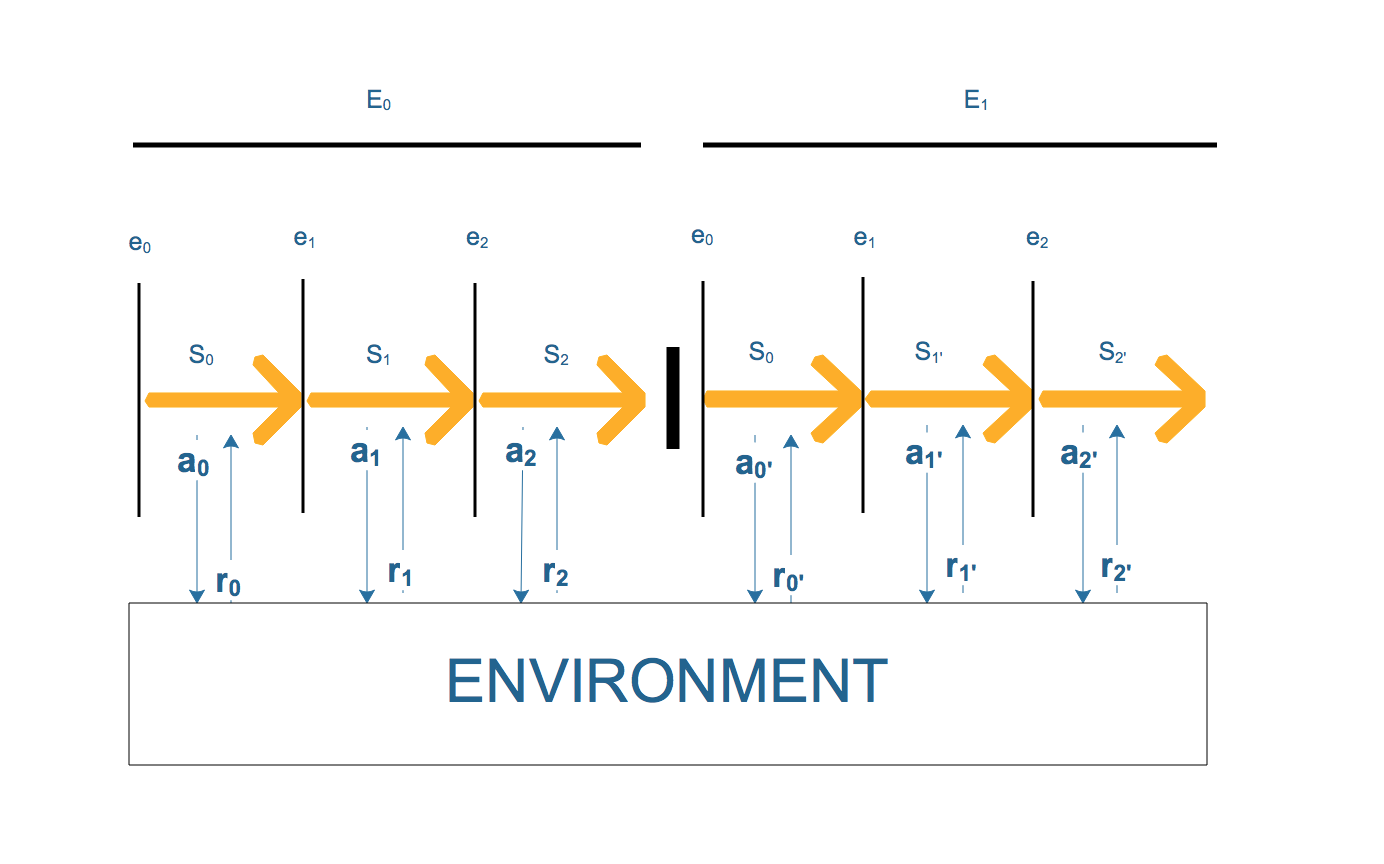
\includegraphics[width= 9cm, height = 5cm]{TrainingModel.png}
    \caption{Schema of an agent-environment interaction broken into two episodes ($E$), each one broken into three epochs ($e$).}
    \label{fig:MDPS}
  \end{figure}
\end{center}

Each episode ends in a special state called \textit{terminal state}, followed by a reset to a starting state or to a sample from a standard distribution of a standard of starting states.

\paragraph{} In many cases the agent environment interaction does not break naturally into identifiable episodes, but goes on continually without limit; we call this \textit{continuing tasks}. The return formulation is problematic for continuing tasks because the final time step would be $T = \infty$, and the return, which is what we are trying to maximize, could itself be infinite~\cite{SuttonBarto}.

\paragraph{} An additional concept that we need is that of \textit{discounting}. According to approach previously explained, the agent tries to select actions so that the sum of the discounted rewards it receives over the future is maximized. In particular, it choses $A_t$ to maximize the expected \textit{discounted return} :

\begin{equation} 
  G_t = R\textsubscript{t+1} + \gamma R\textsubscript{t+2} + \gamma^2 R\textsubscript{t+3} + ... = \sum_{k=0}^{\infty} \gamma^kR\textsubscript{t+k+1}
\end{equation}

where $\gamma$ is a parameter, $0 \eqslantless \gamma \eqslantless 1$, called the \textit{discount rate}. This value determines the present value of future rewards.
If $\gamma < 1$, the infinite sum in (1.5) has a finite value as long as the reward sequence ${R_k}$ is bounded.
If $\gamma = 0$, the agent is "myopic" in being concerned only with maximizing immediate rewards: its objective in this case is to learn how to choose $A_t$ so as to maximize only $R\textsubscript{t+1}$.
As $\gamma$ approaches 1, the return objective takes future rewards into account more strongly~\cite{SuttonBarto}.

\subsection{Policies and Value Functions}
\paragraph{} Almost all reinforcement learning algorithms involve estimating \textit{value functions} that estimate \textit{how good} it is for an agent to be in a given state (or how good it is to perform a given action in a given state). 
More formally we can say that a \textit{policy} is a mapping from states to probabilities of selecting each possible action. If the agent is following policy $\pi$ at time \textit{t}, then $\pi(a|s)$ is the probability that $A_t = a$ if $S_t = s$. 

The \textit{value} of a state \textit{s} under a policy $\pi$, denoted $v_\pi(s)$, is the expected return when starting in $s$ and following $\pi$ thereafter. For MDPs, we can define $v_\pi$ formally by

\begin{equation}
  v_\pi(s) = \mathbb{E}_\pi[G_t | S_t = s] = \mathbb{E}[\sum_{k = 0} ^ {\infty} \gamma^k R\textsubscript{t : k : 1} | S_t = s], \forall s \in S
\end{equation}

where $\mathbb{E}[\cdot]$ denotes the expected value of a random variable given that the agent follows policy $\pi$, and \textit{t} is any time step. We call the function $v_\pi$ the \textit{state-value function} for policy $\pi$.
Similarly, we define the value of taking action \textit{a} in state \textit{s} under a policy $\pi$, denoted $q_\pi(s, a)$, as the expected return starting from \textit{s}, taking the action \textit{a}, and thereafter following policy $\pi$ :

\begin{equation}
  q_\pi(s,a) = \mathbb{E}_\pi[G_t | S_t = s, A_t = a] = \mathbb{E}_\pi[\sum_{k = 0}^{\infty}\gamma^k R\textsubscript{t + k + 1} |S_t = s, A_t = a]  
\end{equation}

We call $q_\pi$ the \textit{action-value function} for policy $\pi$. The value functions $v_\pi$ and $q_\pi$ can be estimated from experience.

A fundamental property of value functions used throughout RL is that they satisfy recursive relationships. For any policy $\pi$ and any state \textit{s}, the following consistency condition holds between the value of \textit{s} and the value of its possible successor states:

\begin{equation}
\begin{split}
  v_\pi(s) = \mathbb{E}_\pi[G_t | S_t = s] \\
           = \mathbb{E}_\pi[R\textsubscript{t+1} + \gamma G\textsubscript{t+1} |S_t = s] \\
           = \sum_{a}\pi(a|s)\sum_{s'}\sum_{r}p(s', r | s, a)[r + \gamma\mathbb{E}_\pi[G\textsubscript{t+1} | S\textsubscript{t+1} = s']] \\
           = \sum_{a}\pi(a|s)\sum_{s', r} p(s', r | s, a)[r + \gamma v_\pi (s')], \forall s \in S
\end{split}
\end{equation} 

where it is implicit that the actions, \textit{a}, are taken from the set $A(s)$, that the next states, $s'$, are taken from the set \textit{S}, and that the rewards, $r$, are taken from the set \textit{R}. 

Equation (1.8) is the \textit{Bellman equation} for $v_\pi$. It expresses a relationship between the value of a state and the values of its successors states~\cite{SuttonBarto}.

\begin{center}
  \begin{figure}[h!]
  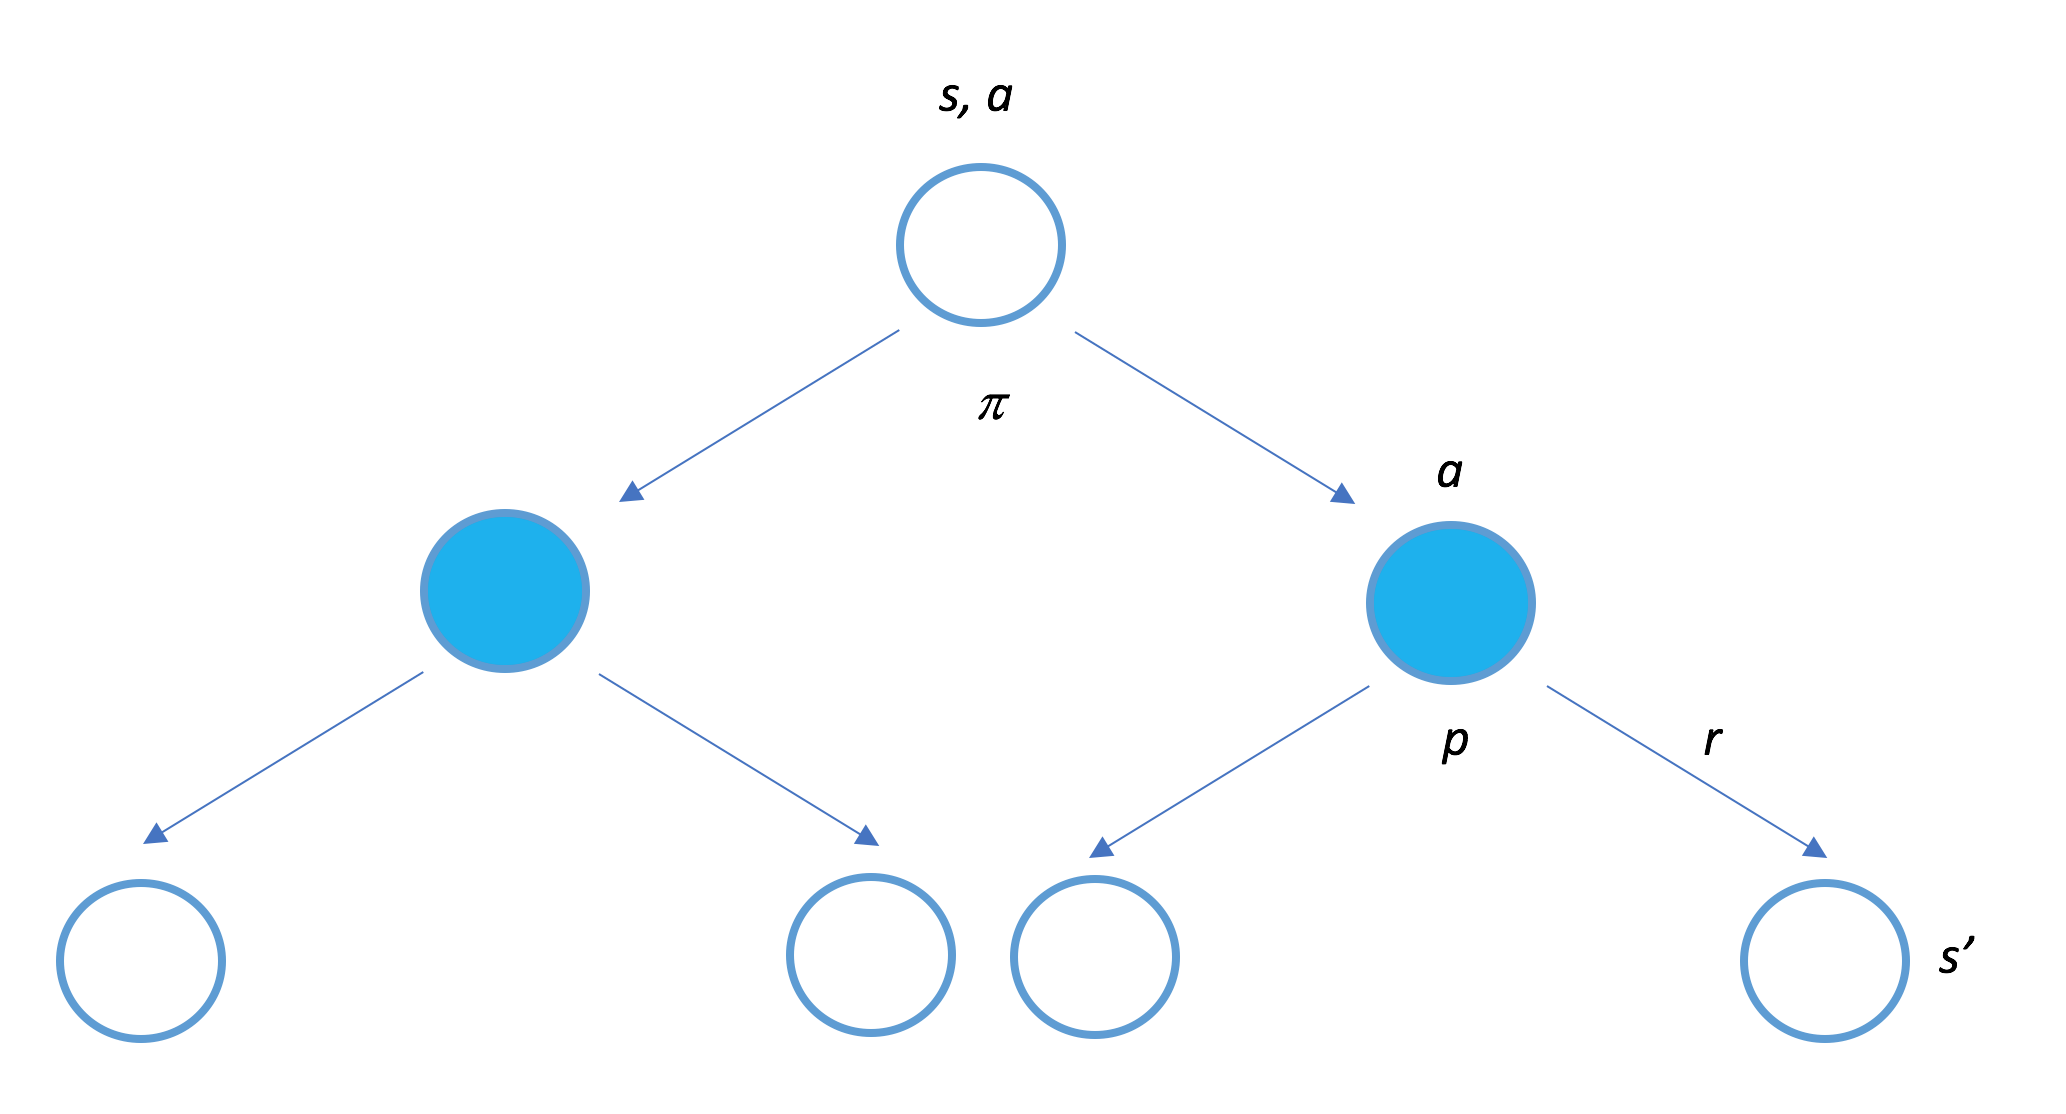
\includegraphics[width= 12cm, height = 6.5cm]{Bellman_graph}
    \caption{Think of looking ahead from a state to its possible successor states. Each open circle represents a state and each solid circle represents a state-action pair. Starting from state \textit{s}, the root node at the top, the agent could take any of some set of actions - two are shown in the diagram - based on its policy $\pi$. From each of these, the environment could respond with one of several next states, $s'$, along with a reward, \textit{r}, depending on its dynamics given by the function \textit{p}. The Bellman equation (1.8) averages over all the possibilities, weighting each by its probability of occurring. It states that the value of the start state must equal the discounted value of the expected next state, plus the reward expected along the way.}
    \label{fig:Bellman_graph}
  \end{figure}
\end{center}

\break \break \break

A policy $\pi$ is defined to be better than or equal to a policy $\pi'$ if its expected return is greater than or equal to that of $\pi'$ for all states. There is always a at least one policy that is better than or equal to all other policies. This is the so called \textit{optimal policy}. We have to underline that it is possible that exist more than one optimal policy. We denote all of them by $\pi_*$. They share the same state-value function, called the \textit{optimal state-value function}, denoted $v_*$, and defined as

\begin{equation}
  v_*(s) = \max\limits_{\pi} v_\pi(s), \forall s \in S
\end{equation}

Optimal policies also share the same \textit{optimal action-value function}, denoted $q_*$ and defined as

\begin{equation}
  q_*(s, a) = \max\limits_{\pi}q_\pi(s, a), \forall s\in S, a\in A(s)
\end{equation}

For the state-action pair $(s, a)$, this function gives the expected return taking action $a$ in state $s$ and thereafter following an optimal policy. Thus, we can write $q_*$ in terms of $v_*$ as follows~\cite{SuttonBarto} :

\begin{equation}
  q_*(s, a) = \mathbb{E}[R\textsubscript{t + 1} + \gamma v_*(S\textsubscript{t+1})|S_t = s, A_t = a].
\end{equation}
